\documentclass[11pt]{article}
\usepackage[T1]{fontenc}
\usepackage{lmodern,microtype,graphicx,amsmath,amssymb,amsthm,booktabs,mathtools}
\usepackage[letterpaper,margin=1in,top=.86in,bottom=.92in]{geometry}
\usepackage[dvipsnames]{xcolor}
\usepackage[colorlinks=true,linkcolor=MidnightBlue,urlcolor=MidnightBlue]{hyperref}
\hypersetup{pdftitle={Beyond Dirichlet GRH at conductors 47 and 71},pdfsubject={One-sided prime estimates and real zeros of dihedral L-functions},pdfauthor={Research note for Vladimir Reshetnikov}}
\usepackage{fancyhdr}
\pagestyle{fancy}\fancyhf{}\lhead{\small\textsc{One-sided prime estimates}}\rhead{\small\textsc{Dihedral Artin factors}}\cfoot{\thepage}
\setlength{\headheight}{14pt}
\setlength{\emergencystretch}{1.5em}
\newtheorem{theorem}{Theorem}
\newcommand{\R}{\mathbb R}
\newcommand{\Q}{\mathbb Q}
\newcommand{\Z}{\mathbb Z}
\newcommand{\dd}{\mathrm d}
\newcommand{\src}[2]{\href{https://github.com/lsernau/grh-lean/blob/72fead102f663d5c7a407964a13dc0cf9d977207/grh/#1}{#2}}
\newcommand{\incoming}[2]{\href{https://github.com/VladimirReshetnikov/ProveIt/blob/5cc267af75a635199ac5d93a7d49cbce521daefc/docs/incoming/#1}{#2}}
\title{\bfseries Beyond Dirichlet GRH at conductors 47 and 71\\[4pt]\large One-sided prime estimates and real zeros of dihedral $L$-functions}
\author{Research note for Vladimir Reshetnikov}
\date{26 November 2026}
\begin{document}
\maketitle
\begin{abstract}
The terminal analytic step of the Lean proof of Dirichlet GRH converts a one-sided estimate at primes into information about zero multiplicities. We give a conductor-$47$ analogue. Either nonprincipal reduced quadratic form of discriminant $-47$ supplies a single upper-bound test for the critical-line conjectures of both two-dimensional Artin factors of the Hilbert class field. Irrational character values prevent cancellation even at a shared zero. The required prime bound remains open. Independently we determine the real zeros, with multiplicities, of every real linear combination of the two completed factors and of all its derivatives. A degree-one modular function on the Fricke quotient makes the Mellin-kernel ratio strictly monotone. The threshold for the original functions is about $1.45202$. At conductor $71$, a rational certificate supplies real-axis positivity for three factors, so a single class again suffices. Their linear combinations admit sharp interpolation with prescribed real zeros and multiplicities. We also determine which pairs of eta factors have a zero-free half-plane of absolute convergence, and give sharp sampling results for the cubic Jensen tests in an earlier ProveIt report.
\end{abstract}

\section{Which part of the Lean argument transfers?}
At commit \texttt{72fead10}, the two editions of \texttt{grh-lean} prove five statements. They include Mathlib's Riemann hypothesis, a zero-location statement for zeta, nonvanishing to the right of $1/2$ for Dirichlet $L$-functions (with the principal pole exception), and versions for zeros of general and primitive characters with the stated trivial-zero exclusions. These are Dirichlet characters over $\Q$. The source of the statements and their final deductions can be read directly in \src{src/Statements.lean}{Statements} and \src{src/Main.lean}{Main}. Andrew Sutherland records kernel replays, independent export checks and comparator runs for the same commit, with only \texttt{propext}, \texttt{Classical.choice} and \texttt{Quot.sound}. We use this published verification and inspected the pinned sources; we did not perform a fresh Lean build. See the \href{https://math.mit.edu/~drew/shortgrh/}{independent verification record} and the accompanying source manifest.

\paragraph{Where the exponent comes from.}
The construction uses Poincar\'e series, chains of theta lifts, and a lattice of integral forms. Short integral forms span with controlled index (A); a second moment provides enough independent forms (B); and the determinant of a chain of lifts bounds the size of integral forms from below (C). The comparison cancels the principal height and leaves $m$ times a prime remainder bounded by $fa(\log b)^5$. Here $m$ is the number of lifts and has size $\sqrt x$. Further normalization gives an error on the scale $(\log b)^6/m$, from which the exponent $-1/2+\epsilon$ follows. The costs and the local divisibility terms are specialized to the chosen fields and twists. See the \src{GUIDE.md}{authors' guide}, \src{src/New/Reduction/MainInequality.lean}{main inequality}, and \src{src/New/Reduction/OneSidedBound.lean}{one-sided bound}.

\paragraph{Where the zeros enter.}
The smoothed prime sums use the weight $1-\chi_K(n)$, a residue class $1\bmod q$, and the kernel $1/n-1/x$ for $n\le x$. The centered transform has a residue proportional to a difference of two sums of zero multiplicities. An auxiliary quadratic twist can be selected so the undesired term has no zero in a prescribed rectangle. Positivity and Landau's singularity principle then turn a one-sided estimate into nonvanishing. The prime weights produced by the lattice carry abelian splitting information. Our application changes these weights and uses a different nonvanishing argument on the real axis. See \src{src/New/Reduction/Zeros/PrimeError.lean}{PrimeError} and \src{src/New/Reduction/Zeros/Criterion.lean}{Criterion}.

\paragraph{Relation to ProveIt.}
The snapshot \texttt{5cc267af} contains 46 incoming ZIPs. Among the relevant predecessors, the \incoming{grh_deficit_transfer_2026-11-25.zip}{deficit report} studies nonabelian Frobenius weights, the \incoming{grh-progression-densities-and-cubic-prime-race.zip}{cubic report} studies $X^3-X-1$, and the \incoming{grh_transfers_density_gaps_and_zero_tests.zip}{density-gaps and zero-tests report} studies $\eta(z)\eta(23z)$ and Gaussian perturbations. The latter already gives finite Jensen-degree ranges at every shift and identifies an obstruction to a general cubic criterion. We use its questions in the appendices. A search of the incoming TeX sources did not turn up the conductor-$47$ classification below. The identity of modular forms that starts the calculation is published. We make no claim of a literature priority determination for the ensuing theorems.

\section{A complete real-zero classification}
Let $K=\Q(\sqrt{-47})$ and let $H$ be its Hilbert class field. The five reduced ideal classes occur in inverse pairs and the principal class. Representatives, up to inversion, are the forms
\[
 Q_0=x^2+xy+12y^2,\qquad Q_1=2x^2+xy+6y^2,\qquad
 Q_2=3x^2+xy+4y^2 .
\]
Reduction gives $(1,1,12),(2,\pm1,6),(3,\pm1,4)$. Thus the class group is cyclic of order five. Complex conjugation acts by inversion, and $\operatorname{Gal}(H/\Q)$ is dihedral of order ten. Put $B_i(z)=\sum_{x,y\in\Z} q^{Q_i(x,y)}$ and $q=e^{2\pi iz}$. Let $\lambda=(1+\sqrt5)/2$ and $\mu=(1-\sqrt5)/2$. The two normalized eigenforms and their difference are
\begin{align}
 f_1&=(B_0-\mu B_1-\lambda B_2)/2, &
 f_2&=(B_0-\lambda B_1-\mu B_2)/2,\nonumber\\
 E(z)&=\eta(z)\eta(47z)=(B_1-B_2)/2=(f_1-f_2)/\sqrt5. \label{eq:eta}
\end{align}
The $L_j$ of these forms are the Hecke $L$-functions of the two inverse pairs of nontrivial ideal class characters, or equivalently the two irreducible nonabelian Artin factors. They have the same gamma factor. See Berkovich and Patane, \href{https://arxiv.org/pdf/1302.2359}{Section 3, equations (3.1)--(3.4)}, and Buzzard, \href{https://www.ma.imperial.ac.uk/~buzzard/maths/research/papers/wt1.pdf}{Section 2.1}. We normalize
\[
 \Lambda_j(s)=\left(\frac{\sqrt{47}}{2\pi}\right)^s\Gamma(s)L_j(s),
 \qquad F_{c}(s)=\Lambda_1(s)-c\Lambda_2(s) \quad(c\in\R).
\]
All these completions are entire. A nonzero multiple of $\Lambda_2$, the one pencil direction omitted by this notation, will have no real zeros.

\begin{theorem}\label{th:real}
For $m\ge0$ let $C_m=\Lambda_1^{(2m)}(1/2)/\Lambda_2^{(2m)}(1/2)$. The thresholds strictly decrease to $1$. The ratio
\[
 R_m(t)=\frac{\Lambda_1^{(2m)}(1/2+t)}
                  {\Lambda_2^{(2m)}(1/2+t)}
\]
is positive and even. It decreases strictly from $C_m$ to $1$ as $t$ increases from zero to infinity, and $R_m''(0)<0$. Consequently the complete list of real zeros of $F_c^{(2m)}$ is as follows.
\begin{center}\begin{tabular}{ll}\toprule
Parameter & Real zeros with multiplicities \\\midrule
$c\le1$ or $c>C_m$ & None\\
$c=C_m$ & One double zero at $s=1/2$\\
$1<c<C_m$ & Two simple zeros, $s=1/2\pm t_c$, $t_c>0$\\\bottomrule
\end{tabular}\end{center}
For all real $s$, $\Lambda_1^{(2m)}(s)>\Lambda_2^{(2m)}(s)>0$.
\end{theorem}

\paragraph{1. Positivity of the smaller kernel.}
For $y\ge1/\sqrt{47}$, $q=e^{-2\pi y}<r=41/100$. The first terms of $f_2$ are $q-\lambda q^2-\mu q^3+\lambda q^4$. The absolute value of the $n$th coefficient is at most the number of ideals of norm $n$ in $K$, hence at most $d(n)\le n$, by the local split, inert and ramified cases. Dropping the positive third and fourth terms gives
\[
 \frac{f_2(iy)}q\ \ge\ 1-\tfrac53r-
 \frac{r^4(5-4r)}{(1-r)^2}>0.04.
\]
The eta product is positive on the imaginary axis, so $f_1(iy)>f_2(iy)$. Poisson summation on each binary lattice gives $B_i(i/(47y))=\sqrt{47}\,y B_i(iy)$: its Gram matrix has determinant $47$ and its adjugate is integrally equivalent to that matrix by rotation. Thus positivity and ordering extend to every $y>0$. This step gives nonvanishing at every real point for both completions by Mellin integration.

\paragraph{2. A modular function with just one pole.}
Define $h(z)=f_2(z)/E(z)$. The weights and characters cancel.
The Fricke transformations of the numerator and denominator agree, by the transformation just proved and \eqref{eq:eta} (then analytic continuation).
Hence $h$ descends to the compact curve $X_0(47)^+=X_0(47)/\langle W_{47}\rangle$. The eta function has no zeros in the upper half-plane. At infinity the numerator begins with $q$ and the denominator with $q^2$. As $47$ is prime, $X_0(47)$ has two cusps, and Fricke exchanges them. Their common image is unramified under this quotient and is the only pole of $h$, of order one. A meromorphic function with one simple pole gives a degree-one isomorphism with the sphere. This proves the coordinate property directly.

There are no elliptic identifications fixing $iy$ for $y>1/\sqrt{47}$. For a determinant-one matrix fixing $iy$ its diagonal entries are equal, and any nonidentity elliptic element has absolute trace less than two (working modulo sign). In $\Gamma_0(47)$ this would force both diagonals zero, inconsistent with the lower-left entry divisible by $47$ and determinant one. In the other coset write the matrix as
\[
 \begin{pmatrix}a&b\\47d&e\end{pmatrix}
 \begin{pmatrix}0&-1/\sqrt{47}\\\sqrt{47}&0\end{pmatrix}.
\]
Equality of diagonals gives $b=-d$, and the trace bound then forces $b=d=0$. The only resulting fixed point is $i/\sqrt{47}$. The quotient map is therefore locally unramified along the open ray. Since $h$ is a degree-one coordinate, $h(iy)$ has nonzero derivative there. It is real and tends to $+\infty$ like $q^{-1}$, so it increases strictly. In particular
\[
 b(u)=\frac{f_1(ie^u/\sqrt{47})}{f_2(ie^u/\sqrt{47})}
 =1+\frac{\sqrt5}{h(ie^u/\sqrt{47})}
\]
is strictly decreasing on $u>0$ and tends to one.

\paragraph{3. The ratio under the Mellin integral.}
Let $K_j(u)=e^{u/2} f_j(ie^u/\sqrt{47})$. The Fricke identities make these positive functions even. Their double exponential decay justifies all differentiations in
\[
 \Lambda_j(1/2+t)=\int_{\R}K_j(u)e^{tu}\,\dd u.
\]
Thus $R_m(t)$ is the expectation of $b(u)$ under the probability density proportional to $u^{2m}K_2(u)\cosh(tu)$ on $u>0$. Its derivative equals the covariance of $b(u)$ and $u\tanh(tu)$. For $t>0$ the second function increases strictly, while $b$ decreases strictly. Integrating $(b(u)-b(v))(u\tanh(tu)-v\tanh(tv))/2$ over two independent draws proves the covariance is strictly negative. At zero the same calculation after a second differentiation gives $R_m''(0)=\operatorname{Cov}(b(u),u^2)<0$. Weighting the measure at zero by $u^2$ proves $C_{m+1}<C_m$.

As $t\to\infty$ at fixed $m$, or $m\to\infty$ at $t=0$, these probability measures escape every compact interval. To check this, compare the mass on $[0,A]$ to that on $[A+1,A+2]$. The ratio tends to zero by the exponential tilt $\cosh(tu)$ or the power tilt $u^{2m}$, respectively. The bounded continuous $b$ tends to one there, so both limits are one. Since the denominator is strictly positive on the real line, strict derivative signs off the center and the strict second derivative at the center prove all the asserted multiplicities.\hfill$\square$

\paragraph{Odd derivatives.}
The real zeros of every odd derivative can be classified as well. For $t>0$, the ratio of derivatives of order $2m+1$ is the expectation of $b(u)$ under the density proportional to $u^{2m+1}K_2(u)\sinh(tu)$. Its derivative is the covariance with $u\coth(tu)$, a strictly increasing function of $u$ because $\cosh v\sinh v>v$ for $v>0$. The ratio decreases strictly from $C_{m+1}$ to $1$, by dominated convergence at zero and the same escape argument at infinity. The central zero of $F_c^{(2m+1)}$ is simple unless $c=C_{m+1}$, when it is exactly triple: its cubic Taylor coefficient is then nonzero because $C_{m+2}<C_{m+1}$. There is one further simple symmetric pair exactly for $1<c<C_{m+1}$. This completes the real-zero classification for all derivative orders.

\paragraph{A limitation illustrated by the same example.}
Taking $c=1$ gives an everywhere positive real completion for $E$. Nevertheless this particular completion has zeros with $\Re s>1$. Indeed $E$ is a combination of distinct Hecke eigenforms with different $T_2$ eigenvalues. Booker and Thorne's theorem for weight-one cusp forms therefore applies. Each such zero recurs in disjoint translates of a small disk by almost periodicity of the absolutely convergent Dirichlet series and Rouch\'e's theorem. The strictly positive Mellin kernel coexists with infinitely many nonreal zeros beyond the critical strip. These belong to the difference of the factors. See \href{https://doi.org/10.2140/ant.2014.8.2027}{Booker and Thorne, Theorem 1.1}.

\paragraph{A rational certificate for the transition value.}
For $h=2\pi/\sqrt{47}$ put $G(a)=\int_1^\infty e^{-av^2}\,dv$.
The substitution $v=e^{u/2}$ in the centered Mellin integral gives
$\Lambda_j(1/2)=4\sum_{n\ge1}a_j(n)G(hn)$.
For $v\ge1$, $v^2\ge1+2(v-1)$, hence
$G(hn)\le e^{-hn}/(2hn)$.
Using $|a_j(n)|\le n$ and $e^{-h}<r=41/100$, the absolute tail after $N=28$,
before multiplication by $4$, is bounded by
$r^{N+1}/(2h(1-r))$. The finite coefficients come from enumerating the three
binary quadratic forms in the theta identities.

For each $a>0$ the program subtracts
$\int_0^1e^{-av^2}\,dv$ from $\tfrac12\sqrt{\pi/a}$.
The integrated Taylor polynomials
$\sum_{k=0}^{m}(-a)^k/[k!(2k+1)]$ are an upper bound at even $m=122$ and a
lower bound at $m=123$, by the sign of the Taylor remainder of $e^{-x}$ for
$x\ge0$. The program evaluates the two endpoints of the interval for $a$
using monotonicity of $G$. It bounds $\pi$ by Machin's arctangent identity,
and all square roots by integer square roots after rational scaling. The
enclosures from \texttt{check\_threshold.py} are
\[
\begin{split}
 0.6660152520&\le\Lambda_1(1/2)\le0.6660152521,\\
 0.4586804524&\le\Lambda_2(1/2)\le0.4586804526,\\
 1.4520244940&\le C_0\le1.4520244943 .
\end{split}
\]
The last line uses the unrounded intervals. For example, the pencil with
$c=7/5$ has two simple real zeros, while the coefficient $3/2$
gives none.

\begin{figure}[ht]
\centering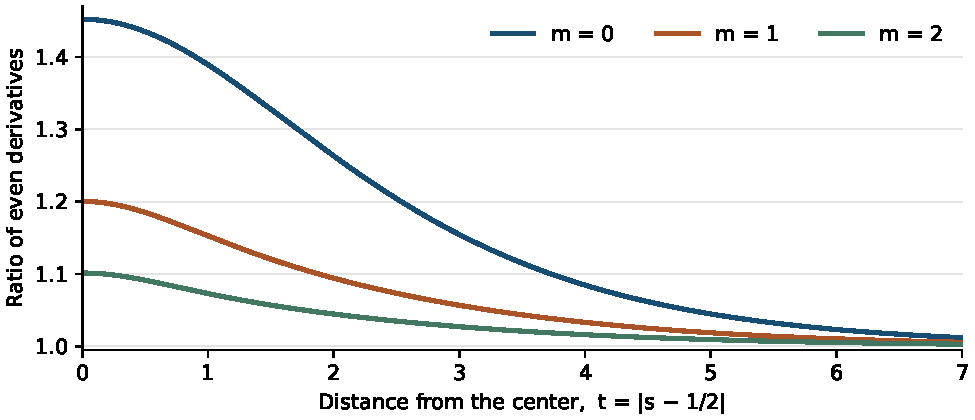
\includegraphics[width=.86\linewidth]{ratios.pdf}
\caption{Conductor $47$. The left endpoint of each curve is the transition for the indicated derivative. Horizontal levels strictly between that endpoint and one meet the curve once on each side of the center, by Theorem~\ref{th:real}. The plot illustrates the proof.}
\end{figure}
\section{One quadratic form detects both critical-line conjectures}
\label{sec:prime}
Choose $Q$ to be either $Q_1$ or $Q_2$, once and for all. Write
\[
 S_Q(x)=\sum_{\substack{p\le x,\ p\ne47\\ p=Q(u,v)\text{ for some }u,v\in\Z}}
   (1-p/x)\log p .
\]
The sum counts each prime once. The appropriate conjugacy class $C$ comprises two of the ten group elements, so the unsmoothed Chebyshev density is $1/5$. The linear smoothing halves the main term.

\begin{theorem}\label{th:primes}
Use the verified Dirichlet GRH for $\zeta$ and $L(s,\chi_{-47})$. For either single choice of $Q$ the following are equivalent.
\begin{enumerate}
\item The nontrivial zeros of both $L_1$ and $L_2$ lie on $\Re s=1/2$.
\item For every $\epsilon>0$ there is $A_\epsilon$ such that, eventually,
\[
                 S_Q(x)\le x/10+A_\epsilon x^{1/2+\epsilon}.
\]
\item The same statement holds with the lower bound
$S_Q(x)\ge x/10-A_\epsilon x^{1/2+\epsilon}$.
\end{enumerate}
In particular either direction of error suffices by itself, and common zeros of the two factors cannot defeat the test.
\end{theorem}

\paragraph{Proof.}
Let $r$ generate the rotations of the dihedral group, labeled so the ideal class of $Q_1$ corresponds to $r$ up to inversion. By ideal class reciprocity, unramified rational primes represented by the form are exactly those with Frobenius in $C=\{r,r^{-1}\}$, or $C=\{r^2,r^{-2}\}$ for the second form. Put $a=(\sqrt5-1)/2$ and $b=-(\sqrt5+1)/2$. For the first class, character column orthogonality gives
\[
 5\mathbf{1}_C=\mathbf 1+\mathrm{sgn}+a\chi_1+b\chi_2 .
\]
Here $\chi_j$ is the Artin character of $f_j$. For the second class interchange $a,b$. In particular $a+b=-1$, and $a,b$ are linearly independent over $\Q$.

Let $U(x)$ sum $\mathbf 1_C(g_p^k)(1-p^k/x)\log p$ over $p^k\le x$, $p\ne47$. Chebyshev's estimate bounds the difference from $S_Q$ by $O(\sqrt x+x^{1/3}\log x)=O(\sqrt x)$. For $\Re s>1$,
\begin{align*}
 \int_1^\infty U(x)x^{-s-1}\,\dd x
 &=\frac{D(s)}{s(s+1)},\\
 5D(s)&=-\frac{\zeta'}\zeta(s)-\frac{L'}L(s,\chi_{-47})
         -a\frac{L'_1}{L_1}(s)-b\frac{L'_2}{L_2}(s)+B(s).
\end{align*}
The ramified correction $B$ is holomorphic on $\Re s>0$, since the finite-image local eigenvalues have absolute value one on inertia invariants. The residue of the integral at $s=1$ is $1/10$. Subtract $1/[10(s-1)]$ and call the resulting meromorphic function $M(s)$. It is regular at every real point of $(1/2,\infty)$ by the Dirichlet input, Theorem~\ref{th:real}, and the cancellation at one. At a candidate nonreal zero $\rho$ with $\Re\rho>1/2$, its residue equals
\[
     -\frac{a\,\operatorname{ord}_\rho L_1+b\,\operatorname{ord}_\rho L_2}
            {5\rho(\rho+1)} .
\]
The numerator can vanish only when both integer multiplicities vanish.

Take $\sigma_0=1/2+\epsilon<1$. Either one-sided estimate supplies a sign and a constant $B_0$ for which
$V(x)=B_0x^{\sigma_0}\pm (U(x)-x/10)$ is nonnegative on $[1,\infty)$, after enlargement on a compact interval. Its Mellin transform continues as $B_0/(s-\sigma_0)\pm M(s)$ and thus is regular on the real interval $(\sigma_0,\infty)$. For completeness, a nonnegative Mellin integrand with finite abscissa $\alpha$ has a singularity there. If regular there, choose a real $s_0>\alpha$ sufficiently close that the Taylor disk of the transform at $s_0$ reaches left of $\alpha$. Evaluating at $s_0-\delta$, the integrated Taylor terms are nonnegative powers of $\delta\log x$ times the integrand. Monotone convergence then gives convergence left of the abscissa, a contradiction. Thus $\alpha\le\sigma_0$ (or convergence holds everywhere). The transform is holomorphic in the open half-plane to its right. The displayed residue excludes all zeros there. Let $\epsilon\downarrow0$ and use the Fricke functional equations to reflect the result.

Conversely Artin factorization gives $\zeta_H=\zeta L(s,\chi_{-47})L_1^2L_2^2$. Under (1) and Dirichlet GRH, effective Chebotarev for this fixed field gives the ordinary weighted count $x/5+O(\sqrt x\log^2(2x))$. Partial integration with $1-p/x$ gives both one-sided estimates. See Greni\'e and Molteni, \href{https://arxiv.org/abs/1709.07609}{An effective Chebotarev density theorem under GRH}.\hfill$\square$

\paragraph{What the arithmetic construction must still do.}
Even in the mean-square sense no rational congruence weight reproduces this class. Let $M$ be any modulus and $v$ any function of a reduced residue class modulo $M$. In the compositum of $H$ and $\Q(\zeta_{\operatorname{lcm}(47,M)})$, the intersection of $H$ with the cyclotomic field is $K$: it contains $K$, and $K$ is the maximal abelian subextension of $H/\Q$. Chebotarev consequently gives a uniform distribution on the five rotations after fixing a compatible residue class that splits in $K$. The conditional probability of $C$ there is $2/5$, and it is zero when the rational prime is inert. The best constant approximation on each fiber is its conditional mean. Therefore
\[
 \lim_{X\to\infty}\frac1{\pi(X)}\sum_{p\le X}^{*}
  |\mathbf1_C(g_p)-v(p\bmod M)|^2\ \ge\
 \frac12\frac25\frac35=\frac3{25}.
\]
The star omits the finitely many excluded primes. Equality is achieved for $M=47$ using that conditional mean. This obstruction concerns substitution of residue weights. It still allows a genuinely new theta-lift construction or cancellations between different arithmetic estimates. For example, an exhaustive enumeration through $10^6$ finds $7{,}819$, $15{,}692$ and $15{,}690$ primes represented by $Q_0,Q_1,Q_2$, respectively, with $47$ omitted. The three disjoint sets exhaust exactly the primes with quadratic symbol $+1$. For the last two classes the centered values $(S_Q(x)-x/10)/\sqrt x$ are about $-0.04823$ and $-0.11582$ at this cutoff. The counts check the identification of the classes and the sample illustrates the normalization. The theorem requires a bound at all sufficiently large $x$.

\section{A real-zero bound at prime levels and sharp interpolation at 71}

Let $p\equiv23\pmod{24}$ be prime and $m=(p+1)/24$.
Let $F$ be a nonzero cusp form with real coefficients, of weight one on
$\Gamma_0(p)$ with quadratic character $\bigl(\frac{-p}{\cdot}\bigr)$.
Assume $F(i/(py))=\sqrt p\,y F(iy)$ for all $y>0$, the positive-sign
Fricke law. This covers the theta eigenforms from nonreal ideal class
characters of $\mathbb Q(\sqrt{-p})$. The corresponding completed
Mellin transform is $\Lambda_F(s)=(\sqrt p/(2\pi))^s\Gamma(s)L(s,F)$,
interpreted by continuation.

\paragraph{Theorem.} For each integer $k\ge0$, the function
$x\mapsto\Lambda_F^{(2k)}(1/2+\sqrt x)$ has at most $m-1$ zeros on
$[0,\infty)$ counted with multiplicity. This entire function of $x$ is
defined by evenness. Equivalently, the $2k$-th derivative has at most
$2(m-1)$ zeros counted with multiplicity on the full real $s$-axis.
At $p=71$, prescribe any two points of $[0,\infty)$ in the $x$-coordinate,
allowing repetition. A unique real linear combination up to nonzero
scalar of the three completed nonabelian class-character factors realizes
exactly that multiset of zeros for $x\mapsto\Lambda_F^{(2k)}(1/2+\sqrt{x})$.
A zero of order $r$ at $x=0$ corresponds to a central zero of order $2r$.

Wei Wang's \emph{Modular $L$-functions and Chebyshev systems} gives the
corresponding geometric and Mellin-transform method and Hermite evaluation
bounds in modular weight at least two
(\href{https://arxiv.org/abs/2611.02933}{Sections 2 and 3, especially Theorem~3.3(ii)}).
Here the eta divisor supplies the geometric bound in weight one. Multiplication
of the integration kernel by $u^{2k}$ gives the same count for every fixed
even derivative.

\paragraph{Divisor bound.}
The eta-quotient criterion applied to $E(z)=\eta(z)\eta(pz)$
uses $p+1\equiv0\pmod{24}$ for both congruences. It gives the same
weight and character as $F$. The eta transformation gives the same Fricke law.
The quotient $F/E$ descends to the compact Fricke quotient $X_0(p)^+$.
The product $E$ never vanishes in the upper half-plane and starts with $q^m$.
There are two cusps on $X_0(p)$, exchanged by Fricke, so $F/E$ has only
one possible pole on the quotient, of order at most $m-1$. It has at most
that many zeros if nonconstant. A nonzero constant quotient has none.

The arc $iy$, $y>1/\sqrt p$, injects into this quotient. Indeed, for
$\left(\begin{smallmatrix}a&b\\c&d\end{smallmatrix}\right)\in\Gamma_0(p)$,
a purely imaginary image of $iy$ requires $ac y^2+bd=0$.
If both terms are nonzero then $ad$ and $bc$ are nonzero and of opposite
signs, incompatible with $ad-bc=1$. Otherwise both products vanish, so the
matrix is diagonal or antidiagonal. The first case is the identity in
$\mathrm{PSL}_2$ and the second is impossible since $p\mid c$.
In the other Fricke coset one first replaces $y$ by $1/(py)$, below the
end of the open arc. Thus $F(iy)$ has at most $m-1$ sign changes on this
open arc.

\paragraph{Passing to the Mellin integral.}
For $u=\log(\sqrt p\,y)>0$ put $K(u)=e^{u/2}F(ie^u/\sqrt p)$.
The centered derivative is $2\int_0^\infty u^{2k}K(u)\cosh(tu)\,du$.
The cusp expansion gives double-exponential decay in $u$.
For $0\le t_1<\cdots<t_l$ and $0<u_1<\cdots<u_l$ one has
$\det[\cosh(t_i u_j)]_{i,j=1}^l>0$.
Indeed, expand each entry using $(t_i^2)^h(u_j^2)^h/(2h)!$,
initially truncating at $h=M$. Cauchy--Binet expresses the determinant as a
sum of products of two generalized Vandermonde determinants with positive
weights. Each product is nonnegative by the alternant formula for
Schur polynomials, and the term using $h=0,\ldots,l-1$ is strictly positive.
This lower bound persists as $M\to\infty$.

The determinant remains strictly positive for repeated nodes in $x_i=t_i^2$
when the rows at a node of multiplicity $r$ are replaced in order by
$\partial_x^j\cosh(\sqrt{x}u)/j!$, $0\le j<r$. To see this, approximate
each repeated node by an increasing cluster of distinct, nonnegative $x$'s,
and divide the determinant by the product of differences within each
cluster. Taylor expansion in $x$ gives the displayed derivative rows in
the limit, including at $x=0$. The lower bound supplied by
$h=0,\ldots,l-1$ contains the full Vandermonde in the $x$'s. After division,
all surviving factors between different clusters have strictly positive
limits. Hence the confluent determinant is also strictly positive.

Let $u_1<\cdots<u_b$ be the sign-change points of $K$. If the transform in
$x$ had $b+1$ zeros counted with multiplicity, take the corresponding rows
of the confluent determinant, with columns at $u_1,\ldots,u_b,u$ and last
point variable. The strict sign of an ordered minor shows that this
determinant alternates sign exactly when $u$ crosses the $b$ points.
Its product with $u^{2k}K(u)$ has constant sign and nonzero integral.
Expansion in the last column gives a linear combination of vanishing
Mellin integrals and their $x$-derivatives, a contradiction.
Differentiation under the integral holds locally uniformly in $x$ by the
double-exponential decay. This also excludes an identically zero transform.

\paragraph{Sharpness at level 71.}
The class group has order seven; its six nontrivial characters yield
three inverse pairs. The three theta eigenforms are linearly independent,
as their $T_2$ eigenvalues are the three distinct numbers
$2\cos(2j\pi/7)$, $1\le j\le3$. Their positive Fricke laws follow from
Poisson summation for their binary theta components.
Berkovich and Patane give the three forms explicitly in
\href{https://arxiv.org/pdf/1302.2359}{Section~4, equations (4.2)--(4.4) and Table~6}.
Two homogeneous linear conditions on the three real coefficients admit
a nonzero solution. For a repeated point the conditions prescribe
vanishing of the value and its first $x$-derivative. The bound $m-1=2$
excludes every additional zero or multiplicity. If the solution space
had dimension at least two, imposing vanishing at another point would
still leave a nonzero solution. This proves uniqueness.

\paragraph{An explicit fourth-order central zero.}
Order the level-$71$ factors as in Berkovich and Patane's equations
(4.2)--(4.4); their $T_2$ eigenvalues in order are
$2\cos(6\pi/7),2\cos(2\pi/7),2\cos(4\pi/7)$.
Let $A=(\Lambda_j(1/2))_{j=1}^3$ and
$B=(\Lambda_j''(1/2))_{j=1}^3$. An exact projective coefficient vector
is $w=A\times B$, and the corresponding completion is
\[
 \mathcal L(s)=\det\begin{pmatrix}
    A_1&A_2&A_3\\ B_1&B_2&B_3\\
    \Lambda_1(s)&\Lambda_2(s)&\Lambda_3(s)
 \end{pmatrix}.
\]
For $k=0$ the interpolation theorem at the repeated node $x=0$ says
that the conditions $w\cdot A=w\cdot B=0$ have a one-dimensional solution
space. Thus $A\times B\ne0$. This combination has vanishing zeroth
and second central derivatives; all odd central derivatives vanish by
symmetry. The zero count proves $\mathcal L^{(4)}(1/2)\ne0$ and excludes every
other real zero of $\mathcal L$. The central cancellation occurs between
the three distinct Artin factors. For orientation, numerical quadrature
with \texttt{example71.py} gives the projective coordinates approximately
$(-0.3172807331,-0.6479315312,1)$. The determinant and zero count provide the
proof independently of these floating-point coordinates.

\subsection*{A second field with the real-zero obstruction removed}
Take the Hilbert class field of $\mathbb Q(\sqrt{-71})$. Reduction of positive definite binary quadratic forms gives seven classes. Representatives up to inversion are
\[
 Q_0=(1,1,18),\quad Q_1=(2,1,9),\quad Q_2=(4,3,5),\quad Q_3=(3,1,6).
\]
Indeed a reduced form has $a\le\sqrt{71/3}<5$; checking $|b|\le a$ gives the displayed classes and their inverses. The group of order seven is cyclic. A prime above $2$ generates it; the square of that prime ideal has norm $4$ and nontrivial class, and the only nonprincipal inverse pair representing $4$ is $Q_2$. This identifies the displayed indices with the respective powers of a generator up to inversion. Complex conjugation gives the dihedral group of order $14$ over $\mathbb Q$.

Put $\Theta_k(iy)=\sum_{x,v\in\mathbb Z}\exp(-2\pi yQ_k(x,v))$, and $q=e^{-2\pi y}$. Grouping integral ideals by their ideal class gives the weight-one Hecke forms
\[
 f_j(iy)=\tfrac12\Theta_0(iy)+
   \sum_{k=1}^3\cos(2\pi jk/7)\Theta_k(iy),\qquad 1\le j\le3.
\]
Here the two units account for the factor $1/2$ before inverse classes are grouped. The constants cancel. For $y\ge1/\sqrt{71}$ one has $q<12/25$; for example $2\pi/\sqrt{71}>37/50$ and the exponential Taylor polynomial of degree four at $37/50$ exceeds $25/12$. On $0<q\le12/25$, respectively, we obtain the uniform lower bounds
\[
             f_1(iy)/q\ge0.999,\qquad f_2(iy)/q\ge0.877,\qquad f_3(iy)/q\ge0.324.
\]
All three bounds are certified by \texttt{check\_level71.py} using rational arithmetic. In detail, let $r_k(n)$ count the representations of $n$ by $Q_k$ and $t=2\cos(2\pi j/7)$. Twice the $n$th coefficient is
$r_0(n)+t r_1(n)+(t^2-2)r_2(n)+(1-t-t^2)r_3(n)$.
The three roots of $t^3+t^2-2t-1$ lie respectively in
$[1.2469,1.2470]$, $[-0.4451,-0.4450]$ and $[-1.8020,-1.8019]$ by sign changes. Enumerate the coefficients up to $N=24$ by
$4aQ(x,v)=(2ax+bv)^2+71v^2$. The coefficients have absolute value at most the number of ideals of norm $n$, at most the divisor count and hence at most $n$. With $r=12/25$, the remaining normalized series has absolute value at most $r^N((N+1)/(1-r)+r/(1-r)^2)$. Interval Horner evaluation on the 24 consecutive intervals of width $1/50$ gives the displayed bounds after subtracting this tail.

Poisson summation gives $\Theta_k(i/(71y))=\sqrt{71}\,y\Theta_k(iy)$: the adjugate of each binary Gram matrix is integrally equivalent to the original matrix by a quarter turn. Thus every $f_j(iy)$ is positive on the whole imaginary axis. Its Mellin integral is positive at every real argument and converges there by rapid decay at both ends. In particular, the three completed $L$-functions are positive throughout the real axis. The one-sided alternative of Section~\ref{sec:rotation} is therefore available: for any one of the three nonprincipal inverse pairs the bound $S_a(x)\le x/14+O_\epsilon(x^{1/2+\epsilon})$ is equivalent, under Dirichlet GRH, to the critical-line conclusion for all three nonlinear factors. The real-axis positivity and its rational certificate are unconditional. The required bound for the prime sum is open.

\section{Further research questions}
\begin{enumerate}
\item Can the Class-$Q_1$ prime weight in Theorem~\ref{th:primes} be realized by a local divisibility contribution of an integral theta lift, with the determinant lower bound retained? Reproducing only its mean $1/5$ supplies no control of its error.
\item At a prime dihedral degree $\ell>7$, the cyclotomic argument below still rules out cancellation. For which explicit fields can the real-axis step be proved by positivity of every constituent's Mellin kernel? This would produce another one-class criterion.
\item Which pairs of equal-conductor newforms admit a quotient with one simple pole after passing to a Fricke quotient? More generally, can one bound the number of real zeros of a linear combination from the number of turns of its kernel ratio when the modular function has degree greater than one?
\end{enumerate}
\appendix
\section{The least nonnegative Frobenius weight}
\label{sec:detector}
The geometric part of the Lean argument attaches nonnegative local amounts to primes. For a nonabelian extension, one can ask how few Frobenius classes a nonnegative replacement must see while giving every nonlinear character a specified coefficient. There is a sharp pointwise answer.

Let $G$ be a finite group, $H=[G,G]$, $e$ its identity, and $d_\pi=\chi_\pi(e)$ for an irreducible complex character $\chi_\pi$. Expand a real class function satisfying $w(g^{-1})=w(g)$ as $w=\sum_\pi a_\pi\chi_\pi$. Character orthogonality gives real coefficients; conjugate characters have equal coefficients. Write $w_*(g)=\mathbf{1}_{H\setminus\{e\}}(g)$.

\paragraph{Pointwise minimum and an exact stability identity.}
Suppose $w\ge0$ and
\[
             -a_\pi\ \ge\ d_\pi/|G| \qquad(d_\pi>1).
\]
Then $w\ge w_*$ pointwise. Equality is attainable simultaneously at every element. More precisely, put $b_\pi=-a_\pi-d_\pi/|G|$ for $d_\pi>1$. For $h\in H$,
\begin{align*}
 w(h)-w(e)-w_*(h)&=
  \sum_{d_\pi>1} b_\pi\bigl(d_\pi-\operatorname{Re}\chi_\pi(h)\bigr),\\
 \frac1{|H|}\sum_{h\in H}\bigl(w(h)-w(e)-w_*(h)\bigr)
 &=\sum_{d_\pi>1} d_\pi b_\pi .
\end{align*}
Thus the average excess on the commutator subgroup measures precisely how much extra weight went into nonlinear coefficients. If all nonlinear coefficients are strictly negative with arbitrary magnitudes, rescaling reduces to the displayed normalization in the nonabelian case. Every such nonnegative detector must count each nonidentity commutator-subgroup element. The minimization concerns coefficients of one prescribed sign; signed prime weights and tests for selected constituents present different problems.

\paragraph{Proof.}
Linear characters equal $1$ on $H$. In $w(h)-w(e)$ they disappear. A unitary matrix of size $d$ has real trace at most $d$. The regular-character identity gives, for $h\in H$,
\[
 \frac1{|G|}\sum_{d_\pi>1}d_\pi(d_\pi-\operatorname{Re}\chi_\pi(h))
    =1-\mathbf{1}_{\{e\}}(h).
\]
These facts give the first equality and the lower bound. Averaging the representation over $H$ projects onto its $H$-fixed vectors. This subspace is $G$-invariant, and a nonlinear irreducible cannot factor through the abelian $G/H$. Thus its averaged trace is zero, giving the second equality. Finally $w_*=\mathbf{1}_H-\mathbf{1}_{\{e\}}$. The first summand has only linear constituents and the second is the regular character divided by $|G|$. Hence $a_\pi(w_*)=-d_\pi/|G|$ for every nonlinear $\pi$. This proves attainment. In particular, every objective $\sum_g c(g)w(g)$ with all $c(g)>0$ has the unique minimizer $w_*$. The result is a finite-group theorem; analytic use of an arbitrary character expansion also requires control of the relevant Artin factors.

\paragraph{Relation to earlier work.}
The \href{https://github.com/VladimirReshetnikov/ProveIt/blob/5cc267af75a635199ac5d93a7d49cbce521daefc/docs/incoming/grh_deficit_transfer_2026-11-25.zip}{incoming deficit report}, section on optimal Frobenius deficits, already constructs $w_*$ and proves its one-sided zero test. Its minimization fixes a combination of permutation characters and varies the abelian correction. Here every nonlinear coefficient can vary independently subject to its lower bound in absolute value. The \href{https://github.com/VladimirReshetnikov/ProveIt/blob/5cc267af75a635199ac5d93a7d49cbce521daefc/docs/incoming/grh_sparse_singular_moduli.zip}{later Frobenius-weight analysis}, in \texttt{frobenius.tex}, already obtains the strict support obstruction and a sharp normalized minimax bound from the same character identities for arbitrary normal subgroups. The display above records the pointwise excess and its average in the normalization used here. We use this as the baseline for the mixed-sign tests. The \href{https://github.com/VladimirReshetnikov/ProveIt/blob/5cc267af75a635199ac5d93a7d49cbce521daefc/docs/incoming/grh-progression-densities-and-cubic-prime-race.zip}{incoming cubic prime-race report} already proves excursions around the $-2/3$ square-term drift for the trace of $X^3-X-1$ on power-spaced grids. Those oscillations are part of the prior work.

\subsection*{An explicit cubic target}
Let $P$ be a monic irreducible cubic in $\mathbb Z[X]$ with nonsquare discriminant, $E$ its splitting field, and $\tau$ the standard representation of $G=S_3$. Exclude the primes dividing the polynomial discriminant. The support of $w_*$ consists of the two three-cycles, so the minimum weight simply asks whether $P\bmod p$ is irreducible. In the order identity, transposition, three-cycle, $\chi_\tau=(2,0,-1)$ and $\mathrm{sgn}=(1,-1,1)$. Hence
\[
                    3w_* =1+\mathrm{sgn}-\chi_\tau.
\]
Define the first Riesz mean of irreducible primes by
\[
 I_P(x)=3\sum_{\substack{p\le x,\ p\nmid\operatorname{disc}(P)\\
                           P\bmod p\ {\rm irreducible}}}
                  \log p\,(1-p/x).
\]
Under the repository's Dirichlet GRH, the following three conditions are equivalent:
\begin{enumerate}
\item All nontrivial zeros of $L(s,\tau)$ have real part $1/2$.
\item $I_P(x)=x/2+O_P(\sqrt{x})$.
\item For each $\epsilon>0$ and sufficiently large $x$, $I_P(x)\le x/2+C_{P,\epsilon}x^{1/2+\epsilon}$.
\end{enumerate}
This is a single-scale Riesz formulation of the earlier deficit principle. The assumed estimate in the last condition remains open already for $P=X^3-X-1$. The classical degree-two factor for this example comes from $\eta(z)\eta(23z)$; see
\href{https://www.sciencedirect.com/science/article/pii/S0723086923000087}{Khare, La Rosa and Wiese, on splitting fields of $X^n-X-1$}.
For general $S_3$, $\tau$ is induced by a nontrivial character of $A_3$. Hecke theory supplies entireness, the functional equation, and the standard zero count for its $L$-function.

\paragraph{Proof of the criterion.}
Write $U(x)$ for the prime-power version with summands $3w_*(g_p^k)\log p(1-p^k/x)$ and $g_p$ a Frobenius element. Chebyshev's bound $\sum_{p\le y}\log p\ll y$ gives $U-I_P=O(\sqrt{x})$; the exponents at least three contribute $O(x^{1/3}\log x)$. For $\operatorname{Re}s>1$,
\[
 \int_1^\infty U(x)x^{-s-1}\,dx=\frac{A(s)}{s(s+1)},\qquad
 A(s)=-\frac{\zeta'}{\zeta}(s)-\frac{L'}L(s,\mathrm{sgn})
                      +\frac{L'}L(s,\tau)+B(s).
\]
Here $B$ removes the finitely many excluded Euler factors and is holomorphic in $\operatorname{Re}s>0$. At $s=1$ the residue of the transform is $1/2$. After centering by $x/2$, at a real zero $\beta>1/2$ of $L(s,\tau)$ the residue is $m_\beta/[\beta(\beta+1)]>0$. Dirichlet GRH excludes poles from the first two $L$-functions in this region, apart from the accounted-for pole at one.

Suppose (3) holds, fix $a=1/2+\epsilon<1$, and make $V(x)=Cx^a-(U(x)-x/2)$ nonnegative by increasing $C$. If the convergence abscissa $\alpha$ of its Mellin transform were greater than $a$, the transform would have a singularity at the real point $\alpha$ by Landau's theorem. Indeed, Taylor-expanding at a real point just to the right of $\alpha$ and using monotone convergence of the integrals of the powers of $\log x$ rules out regularity there. The meromorphic formula gives either a regular point or a simple pole of strictly negative residue. The latter would send the transform to $-\infty$ as $s\downarrow\alpha$, impossible for $V\ge0$. Thus the transform is holomorphic in $\operatorname{Re}s>a$. Every zero there, real or nonreal, would give a pole, since the kernel $1/[s(s+1)]$ never vanishes. Letting $\epsilon$ decrease to zero and applying the functional equation proves (1).

Under (1), all three factors satisfy their respective critical-line theorems. The Riesz explicit formula gives $U(x)=x/2+O_P(\sqrt{x})$. For details, begin with Mellin inversion on $\operatorname{Re}s=2$ and use the full logarithmic derivatives, adding the omitted local terms back at a cost $O_P(\log x)$. Shift to $\operatorname{Re}s=-1/2$ along heights $T$ at distance $\gg_P1/\log T$ from zero ordinates, possible by the unit-interval zero count $O_P(\log T)$. The log derivatives on the horizontal segments are $O_P(\log^2 T)$ by their local partial-fraction expansion. The functional equations and Stirling's formula give $O_P(\log(2+|t|))$ on the new vertical line away from bounded heights. The crossed nontrivial zero residues have absolute sum $O_P(\sqrt{x})$, since the sum of multiplicities times $(1+|\operatorname{Im}\rho|)^{-2}$ converges. At zero the possible double pole costs $O_P(1+\log x)$. This proves (2), which immediately gives (3). A source for the fixed-degree Artin explicit formula and the discriminant-$-23$ example is
\href{https://www.cs.uleth.ca/~nathanng/RESEARCH/phd.thesis.pdf}{N.~Ng, \emph{Limiting distributions and zeros of Artin $L$-functions}, chapters 3--4}.

For a proposed geometric proof this leaves a precise target: control the total excess of the irreducible-prime mean. The support theorem shows what can be gained by changing the character coefficients within the nonnegative construction. The estimate itself still requires cancellation at arbitrarily large scales.

\section{Which rotation classes detect integer zero multiplicities?}
\label{sec:rotation}
Suppose $G=A\rtimes\{1,\iota\}$ with $A$ a nontrivial abelian group of odd order $n$ and $\iota a\iota^{-1}=a^{-1}$. The ordinary dihedral group $D_{2n}$ is the case $A=C_n$. Write a nonidentity rotation class as $[a]=\{a,a^{-1}\}$. In contrast to the fixed-sign condition of Section~\ref{sec:detector}, a single measured class may now have both positive and negative character coefficients. What keeps zero multiplicities from cancelling is their integrality.

Nonlinear irreducible representations of $G$ are the two-dimensional inductions from the nontrivial characters $\psi$ of $A$, indexed by pairs $\{\psi,\psi^{-1}\}$. Indeed the inductions are irreducible by the index-two character calculation, and their squared degrees, together with the two linear characters, sum to $2n$. For a vector of zero multiplicities put $m_1=0$ and write $m_{\psi}=m_{\psi^{-1}}$ for each paired coordinate. The residue seen at the class $[a]$ is proportional to
\[
              T_m(a)=\sum_{\psi\in\widehat A}m_{\psi}\psi(a).
\]

\paragraph{Theorem.}
A collection $\mathcal S$ of nonidentity rotation classes detects every nonzero vector of nonnegative integral multiplicities, in the sense that some $T_m(a)\ne0$, if and only if for every nontrivial cyclic subgroup $C\le A$ it contains the class of a generator of $C$. The least number of classes equals the number of nontrivial cyclic subgroups of $A$. In particular, for ordinary $D_{2n}$ this number is $\tau(n)-1$, where $\tau(n)$ counts positive divisors. For prime $n$, each single nonidentity rotation class suffices.

\paragraph{Proof.}
For any $u$ coprime to the order of $a$, the automorphism $\zeta\mapsto\zeta^u$ of the corresponding cyclotomic field carries $T_m(a)$ to $T_m(a^u)$, since $m_\psi$ is an integer. If every cyclic subgroup has a generator in the measured classes, vanishing there forces $T_m$ to vanish everywhere on $A\setminus\{1\}$. Fourier inversion on $A$ makes all the $m_\psi$ equal; $m_1=0$ forces vanishing.

Conversely, let $C$ be a nontrivial cyclic subgroup with no measured generator. Let $R$ be its set of generators and put
\[
            m_\psi=|R|-\sum_{a\in R}\overline{\psi(a)}.
\]
The inner sum is a rational algebraic integer: it is a sum of roots of unity invariant under every automorphism of the cyclotomic field of order $|C|$, since that group permutes $R$. Hence it is an integer, and it is at most $|R|$ by the triangle inequality. These $m_\psi$ are symmetric, nonnegative integers with $m_1=0$. Character orthogonality gives
\[
             T_m(b)=n|R|\mathbf 1_{\{1\}}(b)-n\mathbf 1_R(b).
\]
Thus $m$ is nonzero and invisible at every measured class. Distinct cyclic subgroups have disjoint generator sets, proving the minimum. For cyclic $A$ the inner sum is a Ramanujan sum. In $C_9$, for example, observation of its generator alone misses the multiplicities $(3,3,0,3)$ at the pairs $\{\pm j\}$ for $j=1,2,3,4$. An additional class of order three gives full detection. The necessity statement is algebraic and makes no prediction that specified Artin factors actually have common zeros with these orders.

\paragraph{Arithmetic consequence.}
Let $E/\mathbb Q$ be a fixed Galois extension with group $G$ as above, and write $L_\psi$ for its induced factors. Each is the Hecke $L$-function of a nontrivial finite-order character over the quadratic field $E^A$, hence entire with the usual functional equation. For unramified rational primes define
\[
 S_a(x)=\sum_{\substack{p\le x\\ \mathrm{Frob}_p\in[a]}}\log p\,(1-p/x).
\]
Assume the repository's Dirichlet GRH and choose one generator class for each nontrivial cyclic subgroup of $A$. Then all $L_\psi$ satisfy RH if and only if for every selected $[a]$ and every $\epsilon>0$,
\[
             S_a(x)=x/(2n)+O_{E,\epsilon}(x^{1/2+\epsilon}).
\]
Under the critical-line conclusion the right side improves to $x/(2n)+O_E(\sqrt x)$. If all the nonlinear factors are known to have no real zeros in $(1/2,1)$, one can use only an upper bound for each centered sum.

To see this, insert all prime powers into $S_a$ at cost $O_E(\sqrt x)$ as in Section~\ref{sec:detector}. The class indicator has coefficient $1/n$ on the trivial character and coefficient $(\psi(a)+\overline{\psi(a)})/n$ on the corresponding nonlinear character. The latter occurs once for each pair. The pole at one therefore contributes $x/(2n)$, and at a zero $\rho$ in the right half of the strip the centered Mellin transform has residue
\[
                    -\frac{T_m(a)}{n\rho(\rho+1)}.
\]
Here $m_\psi$ counts the order of each individual Hecke factor at $\rho$; Dirichlet GRH protects the two linear terms. The two-sided estimate gives holomorphy to the right of $1/2$, so the theorem excludes every such zero. For the converse the Riesz explicit formula of the preceding section applies to each fixed factor and the functional equation supplies the opposite half of the strip. If all the real candidates are already excluded, the transform of a nonnegative majorant minus the centered sum has no real singularity to the right of the proposed exponent. Landau's argument then gives the same holomorphy from the one-sided estimate. This proves the stated transfer without an assumption of linear independence of zero ordinates, simplicity, or disjoint zero sets.

\section{How many shifted Jensen tests detect a polynomial perturbation?}
\label{sec:finite-jensen}
The incoming manuscript \href{https://github.com/VladimirReshetnikov/ProveIt/blob/5cc267af75a635199ac5d93a7d49cbce521daefc/docs/incoming/grh_transfers_density_gaps_and_zero_tests.zip}{\emph{Geometric progressions and nonabelian zero tests}} (files \texttt{jensen.tex} and \texttt{gaussian.tex})
constructs cubic counterexamples to a general kernel criterion while studying
the conductor-$23$ Artin factor. Its Gaussian argument uses every shift of a
cubic Jensen polynomial. For polynomial perturbations there is an exact finite
answer. This calculation determines what evidence from small perturbations
can establish. It does not assume any Riemann hypothesis.

For a real polynomial $V$ bounded below on $[0,\infty)$, consider the even kernel
$K_\epsilon(u)=\exp[-u^2-\epsilon V(u^2)]$, $\epsilon>0$.
Define the coefficients $\gamma_n$ by
\[
 \int_{\mathbb R} e^{zu}K_\epsilon(u)\,du
 =\sum_{n\ge0}\gamma_n z^{2n}/n!,\qquad
 J^{d,n}(X)=\sum_{j=0}^d \binom{d}{j}\gamma_{n+j}X^j .
\]
Call shift $n$ persistent when $J^{3,n}$ is real-rooted along some sequence
$\epsilon\downarrow0$. Each shift may use its own sequence.

\paragraph{Theorem.}
Fix $r\ge3$. For potentials of degree at most $r$, persistence at any
$r-2$ distinct nonnegative integer shifts forces $\deg V\le2$.
In this case all $J^{d,n}$ have negative real roots for every $\epsilon>0$,
$d\ge1$ and $n\ge0$. The test count is sharp. For any set $S$ of $r-3$
nonnegative integers there is a strictly convex increasing polynomial of degree
$r$ whose persistent shifts are precisely $S$. At each fixed shift, the predicted
outcome holds for all sufficiently small positive $\epsilon$.

\paragraph{Proof.}
Set $p=n+1/2$ and let $X_n$ have the gamma distribution of shape $p$
and rate one. The substitution $x=u^2$ and the gamma duplication
formula give $c_n=4^n\gamma_n/\sqrt\pi=\mathbb E e^{-\epsilon V(X_n)}$.
A cubic built from the $c_n$ differs from the original only by positive
rescalings of variable and value. Write $m(n)=\mathbb EV(X_n)$ and
$\Delta m(n)=m(n+1)-m(n)$. The Taylor estimate
$c_n=1-\epsilon m(n)+O_n(\epsilon^2)$ follows by integrating the
pointwise second-order remainder, bounded by a constant times
$\epsilon^2 V^2$ for $0<\epsilon<1$ using the lower bound on $V$.
For the translated cubic $P(W)=\sum_{j=0}^3\binom{3}{j}c_{n+j}(W-1)^j$
the coefficients of $1,W,W^2,W^3$ are, respectively,
\[
 \epsilon\Delta^3m(n)+O_n(\epsilon^2),\quad
 -3\epsilon\Delta^2m(n+1)+O_n(\epsilon^2),\quad
 O_n(\epsilon),\quad 1+O_n(\epsilon).
\]
Thus, if $\Delta^3m(n)\ne0$, its discriminant equals
$-27\epsilon^2(\Delta^3m(n))^2+O_n(\epsilon^3)$.
If $\Delta^3m(n)=0$, it equals
$108\epsilon^3(\Delta^2m(n+1))^3+O_n(\epsilon^4)$.
The transform $V\mapsto m$ takes $x^k$ to the monic polynomial
$(n+1/2)(n+3/2)\cdots(n+k-1/2)$, so is a degree-preserving
linear isomorphism. Hence $r-2$ persistent shifts force the polynomial
$\Delta^3m$, of degree at most $r-3$, to vanish identically.

For the converse take $V(x)=ax^2+bx+c$. For $a>0$, P\'olya's quartic
Fourier integral theorem with arbitrary quadratic coefficient gives only real
zeros for $\int e^{itu}K_\epsilon(u)\,du$.
See N.~G.~de Bruijn, \emph{The roots of trigonometric integrals},
Duke Math.~J.~17 (1950), 197--226,
\href{https://repository.tudelft.nl/file/File_524a4d3c-0858-4c55-b425-8c8ce1fb89da}{p.~197, (1.3)}.
The function $G(w)=\int\cosh(\sqrt w\,u)K_\epsilon(u)\,du$ then
has negative real zeros only. The bound
$|\sqrt w||u|\le (\epsilon a/2)u^4+C|w|^{2/3}$ gives order
at most $2/3$ for $G$. Its genus-zero product places it in the
Laguerre--P\'olya class. For $a=0$, boundedness below gives $b\ge0$
and $G$ is a positive multiple of an exponential with positive slope,
also in that class. Every derivative of $G$ is in the class, so Jensen's
theorem gives real roots for every $J^{d,n}$. Positivity of all the
coefficients puts these roots on the negative real axis.

Finally take $m$ with $\Delta^3m(n)=\prod_{s\in S}(n-s)$, solving by
triangularity of finite differences. Its leading coefficient and that of
the corresponding $V$ are positive. Adding $A x^2$ to $V$ adds $2A$ to
$\Delta^2m(n+1)$ and preserves $\Delta^3m$. Choose $A$ large enough for
$\Delta^2m(s+1)>0$ at each $s\in S$ and $V''>0$ throughout $[0,\infty)$.
The latter is possible since $V''$ has positive leading coefficient.
A further linear adjustment makes $V'(0)>0$. The two discriminant expansions
give all claims. The small-$\epsilon$ thresholds can depend on the shift.
\hfill$\square$

\paragraph{An exact example.}
Take $r=4$ and $V(x)=x^4-14x^3+100x^2+x$. Since
$V''(x)=12(x-7/2)^2+53$, the potential increases from zero and is strictly
convex. Its moment polynomial has $\Delta^3m(n)=24n$ and
$\Delta^2m(1)=95$. Shift zero therefore persists, and each other fixed
shift fails for sufficiently small $\epsilon$. At $\epsilon=10^{-12}$
the checker \texttt{check\_finite.py} bounds the discriminants of the
rescaled cubics using the pointwise inequalities
$1-y\le e^{-y}\le1-y+y^2/2$ for $y\ge0$. Its rational bounds are
\[
 92{,}590{,}000<\operatorname{disc}(P_0)/\epsilon^3<92{,}600{,}000,
 \qquad
 -15{,}553<\operatorname{disc}(P_1)/\epsilon^2<-15{,}551 .
\]

\section{The exact stride for cubic Jensen tests}
The preceding appendix bounds the number of tests when the polynomial degree is known. For continuous $V$ bounded below and of at most polynomial growth, consider testing just one infinite arithmetic progression of shifts. Persistence has the same pointwise-in-the-shift meaning as in Appendix~\ref{sec:finite-jensen}.
\begin{theorem}
If all shifts in $r+2\mathbb N_0$ are persistent for any integer $r\ge0$, then $V$ is a polynomial of degree at most two. For every stride $k\ge3$ and residue $r\bmod k$ there is a smooth strictly convex increasing nonpolynomial $V$ whose persistent shifts are exactly that residue class. Thus one parity, even with an arbitrary finite initial segment missing, detects every nonquadratic perturbation in this class.
\end{theorem}
\begin{proof}
The cubic discriminant expansion in the preceding appendix applies with the stated growth bounds. Persistence implies $\Delta^3m(n)=0$, where $m(n)=\mathbb EV(X_n)$ and $X_n$ has gamma shape $n+1/2$ and rate one.
Form a distribution supported on $[0,\infty)$ by
\[
 T(\phi)=-\int_0^\infty V(x)\frac{\dd^3}{\dd x^3}
       \bigl(x^{r+5/2}e^{-x}\phi(x)\bigr)\,\dd x .
\]
The least exponent at the origin is $r-1/2>-1$. Polynomial growth and exponential decay also let us test $T$ on polynomials and on exponentials $e^{zx}$ for $\Re z<1$. For $j\ge0$ and $p=r+j+1/2$, differentiating the integrand gives
\[
 T(x^j)=\Gamma(p+3)\Delta^3m(r+j).
\]
Indeed the four terms after differentiating have integrals proportional to $m(r+j+3),-3m(r+j+2),3m(r+j+1),-m(r+j)$ with the same factor. Put $F(z)=T(e^{zx})$. This function is analytic on $\Re z<1$ by dominated differentiation. If the progression of stride two is persistent, all even derivatives of $F$ at zero vanish. Hence $F(z)+F(-z)=0$ on $|\Re z|<1$ by analytic continuation. On the imaginary axis this says that $T$ plus its reflected distribution has zero Fourier transform. The distributions are tempered, and their Fourier transforms are the indicated functions (expand the derivative in the defining integral). Fourier uniqueness gives $T+T^{\rm refl}=0$. Their supports meet only at the origin, so $T$ vanishes on $(0,\infty)$. There $T=x^{r+5/2}e^{-x}V'''$ in distributions. The multiplier is smooth and strictly positive. Thus $V'''=0$, forcing a quadratic or lower polynomial, with the value at zero fixed by continuity. Appendix~\ref{sec:finite-jensen} supplies its converse.

For sharpness set $t=\tan(\pi/k)>0$, $h=(1-it)^{-1}$, with $\arg h=\pi/k$, and take
\[
 V(x)=Ax^2+Bx+\cos(tx+\theta).
\]
The gamma expectation of the oscillatory part is $\Re(e^{i\theta}h^{n+1/2})$. Its third difference is $\Re(e^{i\theta}h^{n+1/2}(h-1)^3)$. Choose
$\theta=\pi/2-(r+1/2)\pi/k-3\arg(h-1)$.
Since $h\ne1$, the third difference vanishes precisely at $n\equiv r\pmod k$. The quadratic and linear terms leave it unchanged. The oscillatory contribution to the second difference has absolute value at most $|h-1|^2$, since $|h|<1$. Choose $2A>\max(t^2,|h-1|^2)$ and $B>t$. Then $V'>0$, $V''>0$ and $\Delta^2m(n+1)>0$ everywhere. On the chosen progression the leading discriminant term is positive of order $\epsilon^3$. Off it the leading term is negative of order $\epsilon^2$. This gives the exact set of persistent shifts.
\end{proof}
This sampling statement concerns a perturbative test on a class of kernels; the smallness threshold for $\epsilon$ depends on the shift. The conductor-$47$ zero classification instead holds directly for the arithmetic functions and for every real parameter $c$.

\section{Which two-factor eta products survive the zero test?}
For positive integers $a\le b$, every $f_{a,b}(z)=\eta(az)\eta(bz)$ satisfies
the strict quadratic Jensen inequalities at all shifts, for coefficients from
$G(w)=\Lambda_{a,b}(1/2+\sqrt w)$, where
$\Lambda_{a,b}(s)=(\sqrt{ab})^s\int_0^\infty f_{a,b}(iy)y^{s-1}\,dy$.
Here $J^{d,n}(X)=\sum_{j=0}^d \binom{d}{j}G^{(n+j)}(0)X^j$.
This completed Mellin transform is zero-free in $\operatorname{Re}s>1$ exactly when
\[
                         b/a\in\{1,2,3,5,7,11,23\}.
\]
At every other ratio the transform has infinitely many zeros there, and
at every fixed shift the number of nonreal Jensen roots tends to infinity
as the degree grows. In the coprime
subfamily with $24\mid a+b$, the sole surviving pair is $(1,23)$.

\paragraph{Proof.}
A common dilation leaves this normalized completion invariant, by a change of variables in the integral.
First divide $a,b$ by their gcd. Now set $g=\gcd(a+b,24)$, $r=24/g$,
$A=ra$, $B=rb$, $N=AB$ and $m=(a+b)/g$. Both eta congruence sums for
$f_{A,B}$ at level $N$ equal $A+B=24m$ (count both factors when $A=B$).
The cusp-order formula has positive summands. Thus this is a weight-one
cusp form of character $\chi(d)=(\frac{-AB}{d})$; see
K.~Ono, \emph{The Web of Modularity}, Theorems 1.64--1.65.
Its Fourier expansion starts with $q^m$ with coefficient one; denote its
coefficients by $a_n$. We have $\gcd(m,N)=1$ since $a+b$ is coprime to
$ab$ and $m$ is coprime to $r$.
If $m>1$, the coefficient of $q$ in $T_m f_{A,B}$ is $a_m=1$ whereas
$a_1=0$. This rules out an eigenfunction for all good-prime $T_p$,
which generate $T_m$ by the Hecke relations.

If $m=1$, $(A,B)$ is one of the twelve two-part partitions of $24$ and
$a_1=1$. The four pairs $(5,19),(7,17),(9,15),(11,13)$ have $a_2=a_4=0$;
the pair $(10,14)$ has $a_3=a_9=0$. The chosen prime $p$ in each case
is coprime to $N$, so the eigenform relation $a_{p^2}=a_p^2-\chi(p)$ fails.
The remaining seven are the classical multiplicative weight-one eta
eigenforms. Their ratios give the set displayed above, and the absolutely
convergent Euler products give nonvanishing on $\operatorname{Re}s>1$.
See Dummit, Kisilevsky and McKay, \emph{Multiplicative products of
$\eta$-functions}, Contemp. Math. 45 (1985), 89--98, and
\href{https://www.numdam.org/item/10.5802/jtnb.495.pdf}{Voskresenskaya, section 2}
for the explicit eigenform list. By
\href{https://research-information.bris.ac.uk/ws/files/95488278/mf_zeros_revised.pdf}
{Booker--Thorne, Theorem 1.1 and Remark (2)}, each excluded form
has infinitely many zeros in $\operatorname{Re}s>1$.

For the Jensen claim, center the Mellin kernel by putting $y=e^u/\sqrt{ab}$.
Apart from a positive constant its logarithm is
$h(u-v)+h(u+v)$, with
$h(t)=t/4+\log\eta(ie^t)$ and $v=\tfrac12\log(b/a)$.
The all-shift quadratic result follows from the paired-eta curvature estimate
of the incoming \texttt{jensen.tex}. For clarity, its derivative estimate uses
the term $-2\pi e^t/24$ and the terms
$-\sigma_{-1}(k)e^{-2\pi k e^t}$ in the expansion of $h$ for $t\ge0$.
For $Y=2\pi k e^t>6$ the fourth derivative of $e^{-Y}$ equals
$e^{-Y}Y(Y^3-6Y^2+7Y-1)>0$.
Eta inversion makes $h$ even, so $h^{(4)}<0$ on the real axis.
For the even logarithm $g$ of the centered kernel this gives
$(g(\sqrt{x}))''<0$ for $x>0$, by integrating $g^{(4)}<0$ first
to obtain $g'''(u)<0$ and then $(ug''-g')'=ug'''<0$ for $u>0$.
The normalized Mellin moments of $e^{g(\sqrt{x})}$ are strictly
log-concave: writing $M_p=\int_0^\infty x^{p-1}e^{-V(x)}dx$ with
$V(x)=-g(\sqrt{x})$, the expectation of $V'$ under the density
$x^p e^{-V(x)}/M_{p+1}$ equals $pM_p/M_{p+1}$ by integration
by parts. This expectation strictly increases with $p$ in steps of one
because weighting a positive density by $x$ increases the mean of the
strictly increasing $V'$ (by strict positive covariance).
The moments $M_{n+1/2}/\Gamma(n+1/2)$ give the Jensen coefficients
up to a constant and a geometric factor.

\paragraph{Failure in every shift.}
Use the normalized modular form $f_{A,B}$, whose completed transform is
$E(s)L(s)$ with $E(s)=(\sqrt{N}/2\pi)^s\Gamma(s)$. The completion above
is invariant under common dilation, by substitution in the Mellin integral.
For every excluded pair choose a closed disk $D\subset\{\operatorname{Re}s>1\}$
with a zero of $L$ inside and none on its boundary. Absolute convergence of
the Dirichlet series gives arbitrarily large $t_j$ with
$L(s+it_j)\to L(s)$ uniformly on $D$. Indeed truncate the series uniformly,
and simultaneously approximate the phases $n^{-it_j}$ by one for the
finitely many indices retained. Every fixed derivative of $L$ is uniformly
bounded on the corresponding vertical strip by absolute convergence slightly
to its left.

Put $w=(s-1/2)^2$ and fix $n\ge0$. Uniformly on $D+it_j$ as $j\to\infty$,
\[
 \frac{[2(s-1/2)]^n G^{(n)}(w)}{E(s)(\log s)^n}
 =L(s)+O_n(1/\log t_j).
\]
To verify this, expand $d/dw=[2(s-1/2)]^{-1}d/ds$ repeatedly.
After the displayed power of $2(s-1/2)$ is applied, the leading term
is $(E L)^{(n)}$; the terms with $k<n$ derivatives have coefficients
$O_n(|s|^{k-n})$. Stirling's differentiated formula gives
$E^{(k)}/E=(\log s)^k+O_k((\log|s|)^{k-1})$ for $k\ge1$ on this strip.
Leibniz's rule proves the estimate. All normalizing factors are nonzero
on the translated disks for large $j$.
Rouch\'e's theorem now gives a zero of $G^{(n)}((s-1/2)^2)$ in every
sufficiently large translated disk. Choose the disks disjoint with increasingly
large positive ordinate: their squares about $1/2$ lie off the real axis and
give infinitely many distinct zeros of $G^{(n)}$.
Finally $J^{d,n}(w/d)\to G^{(n)}(w)$ locally uniformly as $d\to\infty$,
by termwise binomial scaling and domination by the absolute Taylor series.
Any finite collection of disjoint small disks around nonreal zeros must
therefore contain zeros of every sufficiently large scaled polynomial.
This proves the asserted divergence of the nonreal root count.

In fact the number of nonreal roots is $\gg_{a,b,n}\log d/\log\log d$.
To see this, a fixed sufficiently good uniform approximation on $D$ suffices
for Rouch\'e. The corresponding shifts are relatively dense: a finite
Dirichlet sum approximates $L$ uniformly, and the returns of its phase flow
to any neighborhood of the identity have bounded gaps by compactness
of the closure of the flow in its finite torus.
We can therefore choose $\gg T$ disjoint translated disks at heights
between $T/2$ and $T$. On their boundaries the derivative estimate and
Stirling's formula give $|G^{(n)}((s-1/2)^2)|\ge e^{-2T}$ for large $T$.
All the squared disks lie in $|w|\le R$ with $R=O(T^2)$.
Writing the binomial scaling coefficient as
$u_{d,j}=\prod_{k=0}^{j-1}(1-k/d)$ for $j\le d$ and zero otherwise gives
$0\le1-u_{d,j}\le j(j-1)/(2d)$. Positivity of the Taylor coefficients yields
\[
 \max_{|w|\le R}|G^{(n)}(w)-J^{d,n}(w/d)|
 \le R^2G^{(n+2)}(R)/(2d)\le e^{C_nT\log T}/d .
\]
For the last inequality, the centered eta kernel is bounded by
$C\exp(-c e^{|u|})$ from its product and symmetry. Thus
$\log\max_{|w|\le R+1}|G(w)|=O(\sqrt{R+1}\log(R+2))$ by its
Mellin integral (or the gamma integral after substituting $e^{|u|}$).
Cauchy's bound on a unit circle gives the same growth bound for the
fixed derivative. With $T=c_n\log d/\log\log d$ and $c_n$ sufficiently
small, the approximation error is at most $d^{-1/2}<e^{-2T}$.
A second application of Rouch\'e transfers all these disks to the
degree-$d$ polynomial. The constants depend on the eta product and shift.

\end{document}
